\subsection{Administrationssystem}
I det følgende afsnit kan der læses om integrationstest for \gls{AS}.

\textbf{Introduktion}\\
Der er lavet integrationstests der tager udgangspunkt i ViewModels og tester med forskellige andre klasser, bl.a. fra \gls{SL} og andre klasser i \gls{AS}.\\

\textbf{Testdetaljer}\\
Testene er foretaget ved hjælp af NUnit og NSubstitute. Funktionaliteten i viewmodels er testet sammen med modeller fra \gls{AS}et selv, samt \gls{SL}. For at finde ud af, hvilke klasser der skulle testes sammen er der udarbejdet et dependency tree, som kan ses på figur \ref{fig:AS-dependencies}.\\

\newpage
\textbf{Dependency tree}
\begin{figure}[H]
	\centering
	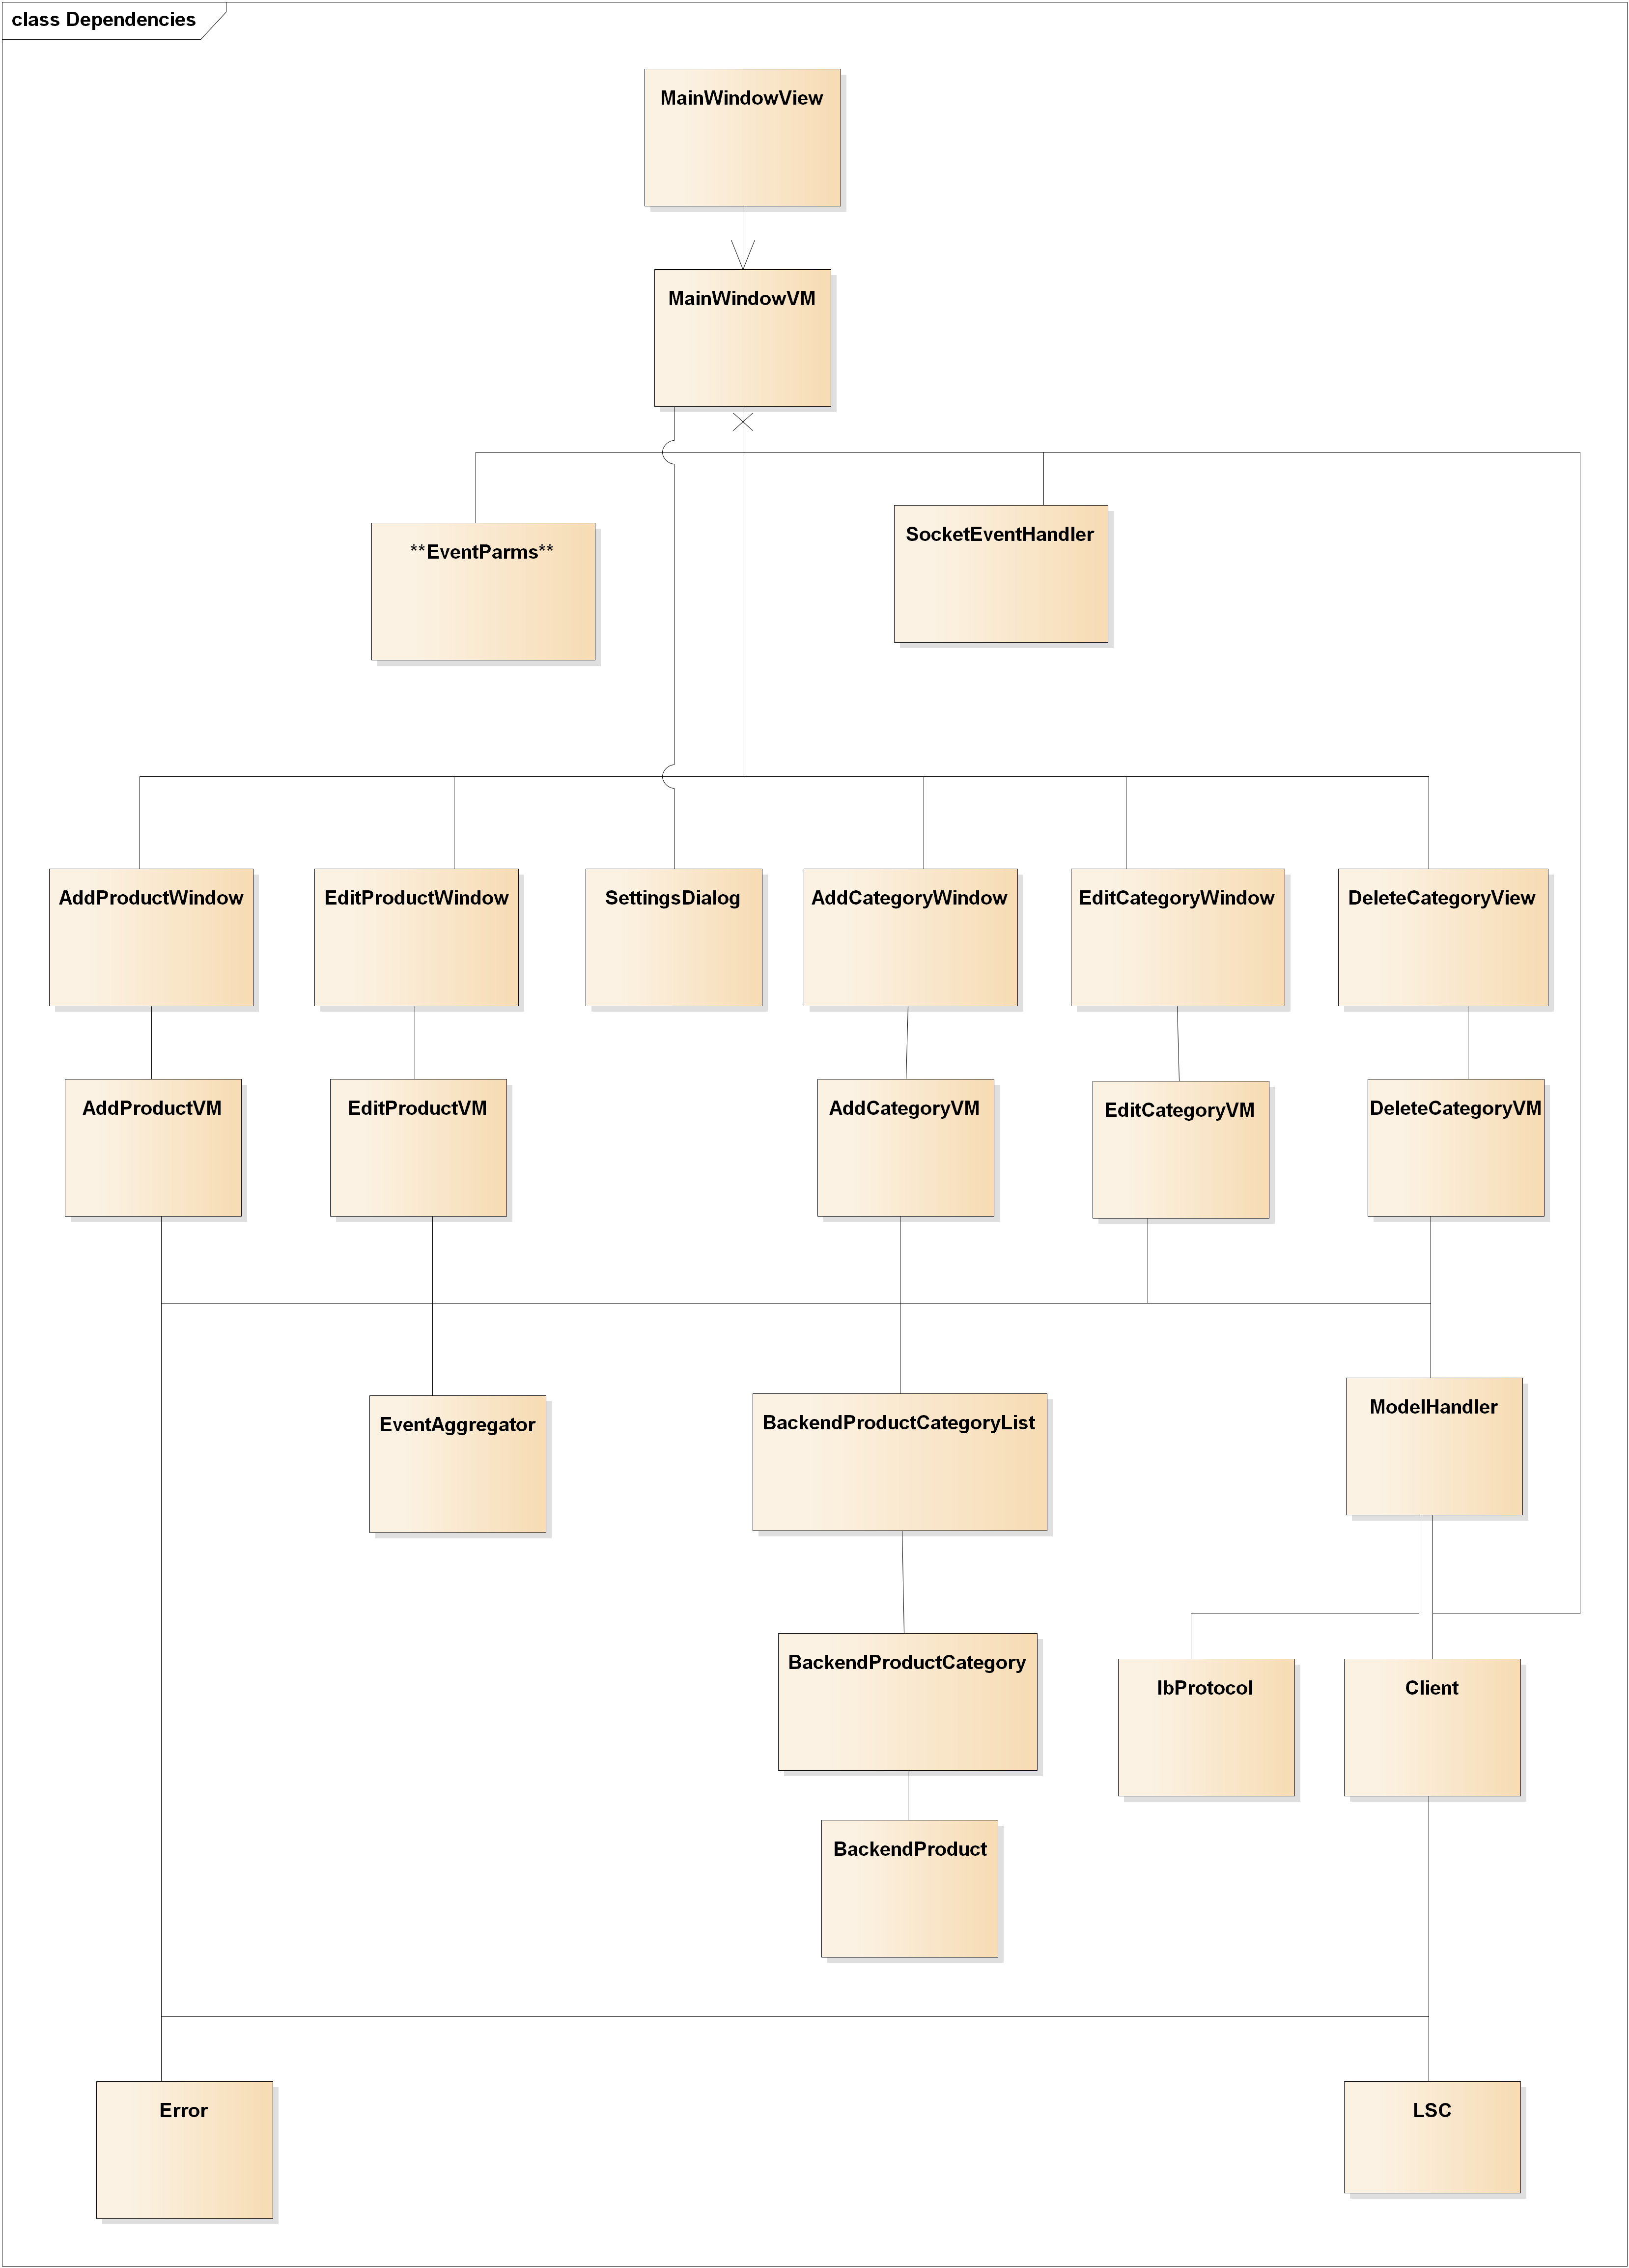
\includegraphics[width=1\textwidth]{Test/Integrationstest/Images/AS-Dependencies}
	\caption{Dependency tree for \gls{AS}}
	\label{fig:AS-dependencies}
\end{figure}

\textbf{Beskrivelse af integrationstest}\\
Som det kan ses er det et rimelig omfattende dependency tree. Alle views (Window klasserne) er udelukket fra testen, da det blot er XML kodning af vinduernes udseende og data bindinger. Alle vinduerne afhænger af deres viewmodel. Disse viewmodels indeholder den bagvedliggende funktionalitet, i samarbejde med models. Disse er derfor testet sammen. Testene er foretaget så de tester den funktionalitet en bruger ville benytte sig af i brugergrænsefladen. Dette indebærer stort set bare at teste de kommandoer som knapperne i en GUI benytter sig af, samtidig med at der foretages ændringer i de datamodeller som ligger i de forskellige viewmodels. Testene er foretaget ud fra et "top-down" princip, hvor de øverste klasser (viewmodels) er testet med de klasser de afhænger af (models, såsom BackendProductCategoryList, ModelHandler, og så fremdeles).